% Beamer slides – Fantasy Football Optimization Project
% Author: Marco De Rito
\documentclass[aspectratio=169]{beamer}

% ------------------------------------------------------------------ %
% Theme and colours 
\usetheme{Madrid}
\usecolortheme{seagull}
\usefonttheme{professionalfonts}

% ------------------------------------------------------------------ %
% Packages
\usepackage[utf8]{inputenc}
\usepackage[T1]{fontenc}
\usepackage[english]{babel}
\usepackage{tikz}
\usepackage{pgfplots}
\pgfplotsset{compat=1.18}   % o la versione che hai installato
\usetikzlibrary{positioning,patterns} % opzionale ma utile

\usepackage{graphicx}
\usepackage{subcaption}
\usepackage{amsmath}
\usepackage{booktabs}
\usepackage{siunitx}
\usepackage{colortbl}
\usepackage{listings}   % code snippets
\setbeamertemplate{navigation symbols}{}
\lstdefinestyle{mystyle}{
	basicstyle=\ttfamily\footnotesize,
	backgroundcolor=\color{gray!10},
	frame=single,
	keywordstyle=\color{blue},
	commentstyle=\color{green!50!black},
	breaklines=true,
	numbers=left,
	numberstyle=\tiny\color{gray},
	captionpos=b
}
\lstset{style=mystyle}

% ------------------------------------------------------------------ %
% Custom commands
\newcommand{\fitness}{\mathcal{F}}
\newcommand{\pen}{\mathrm{Penalty}}
\newcommand{\score}{\mathrm{Score}}
\newcommand{\bids}{\mathbf{b}}

\lstset{
	language=Python,
	basicstyle=\ttfamily\small,
	breaklines=true,
	frame=single,
	columns=fullflexible
}

% ------------------------------------------------------------------ %
\title[Evolving Bids]{Evolving Bids for a Fantasy-Football Auction\\
	\small Metaheuristics and Inverse Optimization in a Multi-Manager Setting}

\author{Marco De Rito}
\institute{University of Trieste}
\date{2024/25}

\begin{document}
	
	\begin{frame}[plain]
		\titlepage
	\end{frame}
	
	\begin{frame}{Agenda}
		\tableofcontents
	\end{frame}
	
	\section{Problem Statement}
	\begin{frame}{Problem Statement}
		\scriptsize
		\begin{block}{Goal}
			Optimise a multi–manager fantasy-football auction by evolving a
			vector of \alert{bids} that maximises total team score while
			satisfying \emph{all} hard constraints.
		\end{block}
		
		\begin{columns}[T,onlytextwidth]
			\column{0.5\textwidth}
			\textbf{Notice legend}
			\vspace{0.3em}
			\begin{tabular}{@{}ll@{}}
				$B$ & current budget of \emph{one} manager\\
				$b_i$ & bid placed by that manager for player $i$\\
				$N_{\max}$ &  squad size\\
				$N_{\text{rem}}$ & empty slots still to be filled\\
				$m_r, M_r$ & min / max players for role $r$\\
				$r$ & role index: P, D, C, A\\
			\end{tabular}
				\textbf{Constraints}
			\begin{itemize}
				\item Bid domain $b_i \in \{0\} \cup [1, \infty)$
				\item Turn budget $\sum_i b_i \le B$
				\item Per-player cap $b_i \le 0.4B$
				\item Reserve credits $B - \sum b_i \ge N_{\text{rem}}$
				\item Squad size $|\text{team}| = N_{\max}$
				\item Role quotas enforced every turn
			\end{itemize}
			
			\vspace{1em}

			\column{0.48\textwidth}
			\textbf{Inputs}
			\begin{itemize}
				\item Initial budget per manager $B$  (CLI)
				\item Number of managers (CLI)
				\item Algorithm for each manager $r \in \{PSO, DE, ES\}$ (CLI)
				\item  squad size $N_{\max}$ (CLI)
				\item Role quotas $(m_r, M_r)$ for $r \in \{P, D, C, A\}$ (CLI)
				\item Data set: 600+ Serie A players (23/24 stats)
			\end{itemize}
			
			
		\end{columns}
	\end{frame}
\section{Software Architecture}
\begin{frame}{Project Files}

	\begin{block}{}
		Logical separation between data, logic, optimization and output.
	\end{block}
		\vspace{0.3em}
		\textbf{Main Modules}
		\begin{itemize}
			\item \texttt{main.py} – CLI input \& full pipeline control
			\item \texttt{data\_loader.py} – loads \& cleans player data
			\item \texttt{utils.py} – defines \texttt{Player}, \texttt{Manager}, \texttt{score\_player}
			\item \texttt{optimization.py} – implements PSO, DE, ES + auction logic
			\item \texttt{report\_generator.py} – generates PDF report
		\end{itemize}
		\vspace{0.3em}
		\textbf{Tuning Scripts}
		\begin{itemize}
			\item \texttt{hyperparameter\_tuning.py}
			\item \texttt{inverse\_param\_tuning.py}
		\end{itemize}
		\vspace{0.3em}
		\textbf{Supporting Files}
		\begin{itemize}
			\item \texttt{Fantacalcio\_stat.csv}, \texttt{requirements.txt}, \texttt{.git/}, \texttt{venv/}
		\end{itemize}
		

\end{frame}
\begin{frame}{Architecture}


		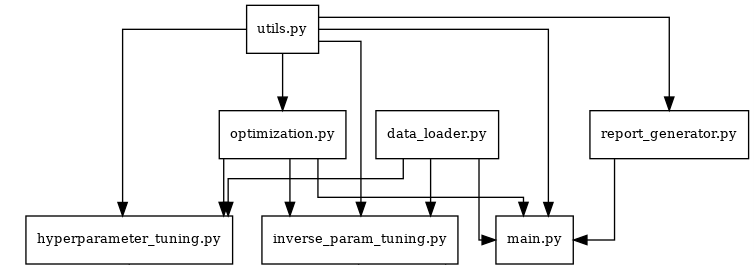
\includegraphics[width=0.90\textwidth]{plot/architecture_diagram.png}

\end{frame}

	
	
	
	\section{Representation}
	\begin{frame}{Genotype vs Phenotype}
		\begin{columns}[T,onlytextwidth]
			\column{0.48\textwidth}
\textbf{Genotype}
\begin{itemize}
	\item Continuous bid vector: $\bids = (b_1, b_2, \dots, b_n)$
	\item Index \(i\) is bound to a fixed player
	\item Crossover / mutation touch numerical values only
	\item \textit{Example: } $(30.5, 0, 7.8, \dots, 0)$
\end{itemize}

			
			\column{0.48\textwidth}
			\textbf{Phenotype}
			\begin{itemize}
				\item Simulated squad obtained from \(\bids\)
				\item Includes roles, spent budget, expected score
				\item Graded via fantasy-football scoring rules
			\end{itemize}
		\end{columns}
	\end{frame}
	

	
\section{Algorithmic Formulas}
\begin{frame}{Algorithmic Formulas \& Parameters}
	\scriptsize
	\renewcommand{\arraystretch}{1.1}
	\begin{columns}[T,onlytextwidth]
		% Colonna di sinistra: formule
		\column{0.55\textwidth}
		\textbf{Particle Swarm Optimization (PSO)}
		\[
		\mathbf{v}_i^{t+1} =
		\omega \mathbf{v}_i^{t} +
		c_1 r_1 (\mathbf{p}_i - \mathbf{x}_i^{t}) +
		c_2 r_2 (\mathbf{g} - \mathbf{x}_i^{t})
		\]
		\[
		\mathbf{x}_i^{t+1} = \mathbf{x}_i^{t} + \mathbf{v}_i^{t+1}
		\]
		
		\textbf{Differential Evolution (DE)}
		\[
		\mathbf{y} =
		\mathbf{x}_a + F (\mathbf{x}_b - \mathbf{x}_c)
		\]
		\[
		z_j =
		\begin{cases}
			y_j & \text{if } r_j < CR \text{ or } j = j_{\text{rand}} \\
			x_{i,j} & \text{otherwise}
		\end{cases}
		\]
		
		\textbf{Evolution Strategies (ES)}
		\[
		\mathbf{x}_{\text{child}} = \mathbf{x}_{\text{parent}} + \sigma \mathcal{N}(0, I)
		\]
		{\tiny(best $\mu$ of parents + offspring survive)}
		
		% Colonna di destra: tabella
		\column{0.45\textwidth}
		\textbf{Algorithm Parameters}
		\vspace{0.3em}
		\small
		\begin{tabular}{@{}llll@{}}
			\toprule
			Alg. & Param. & Desc. & Val.\\
			\midrule
			PSO & $\omega$ & inertia & 0.7\\
			PSO & $c_1$ & cog. & 1.8\\
			PSO & $c_2$ & soc. & 1.8\\
			DE  & $F$   & diff. w. & 0.5--1.0\\
			DE  & $CR$  & cross.  & 0.7\\
			ES  & $\mu$ & parents & 40\\
			ES  & $\lambda$ & offspr. & 80\\
			\bottomrule
		\end{tabular}
	\end{columns}
\end{frame}

	
	\section{Fitness}
	\begin{frame}[fragile]{Fitness Function}
		\[
		\fitness(\bids) = \pen(\bids) - \sum_{i \in \mathcal{A}(\bids)} w_i \score_i,
		\qquad
		\mathcal{A}(\bids) = \{i \mid b_i \ge \text{thr}\}
		\]
		\vspace{-1ex}
		\begin{itemize}\small
			\item $\pen$ mixes \emph{budget leftover}, missing roles, squad size errors
			\item $w_i$ doubles if the role is currently under-represented
			\item Minimisation problem: lower \(\fitness\) \(\leftrightarrow\) stronger squad, fewer violations
			\item $thr=1$ 
			
		\end{itemize}
			\begin{lstlisting}[language=Python, caption={Function score}, style=mystyle]
def score_player(player):
	goals       = getattr(player, 'goals_scored', 0)
	....
	matches     = getattr(player, 'matches_played', 0)
	return (0.5 * goals + 0.2 * assists - 0.05 * yellow - 0.1 * red + 0.2 * rating + 0.2 * pens - 0.5 * conceded + 0.5 * saved + 0.5 * matches)
		\end{lstlisting}

	\end{frame}
	
	\section{Conflict Resolution}
	\begin{frame}[fragile]{Auction Conflict Heuristic}
		\begin{enumerate}\footnotesize
			\item Gather all bids $(\text{mgr}, \text{player}, b)$
			\item Group by player
			\item Single bidder $\Rightarrow$ immediate assignment
			\item Otherwise:
			\begin{itemize}
				\item Sort bids $b_1 \ge b_2 \ge \dots$
				\item If $b_1 - b_2 > g_{\text{trigger}}$ $\Rightarrow$ highest wins
				\item Else launch up to 5 dynamic rebids\\
				\smallskip
				\textit{\footnotesize (rebids = recompute bids with small noise or fallback threshold)}
				
			\end{itemize}
		\end{enumerate}
		\begin{lstlisting}[language=Python, caption={Semplified Dynamic rebid heuristic}, style=mystyle]
# Inputs: b1 = top bid, b2 = second bid, B = second manager's remaining budget, n = number of players still needed
ratio = B / n
gap = b1 - b2
#Compute dynamic rebid increment
dynamic_inc = max(1, int(round(gap / 2 * ratio))) + 1
# Apply rebid
b2 += dynamic_inc
		\end{lstlisting}
		
	\end{frame}
	
	\section{Example}
\begin{frame}{Example: Manager and Player Distributions}
	\centering
	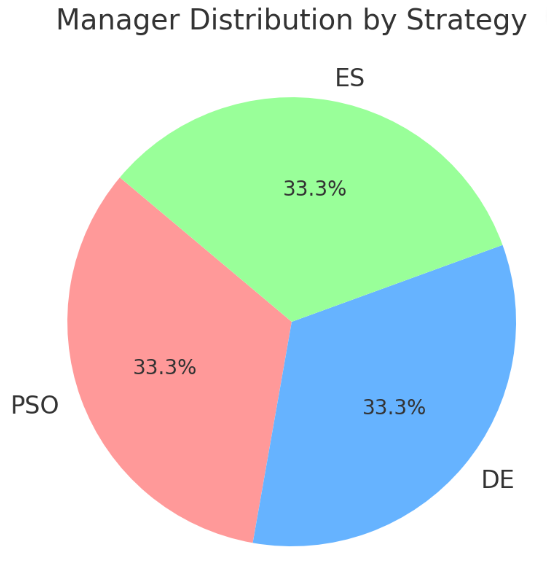
\includegraphics[width=0.45\linewidth]{plot/manager_distribution.png}
	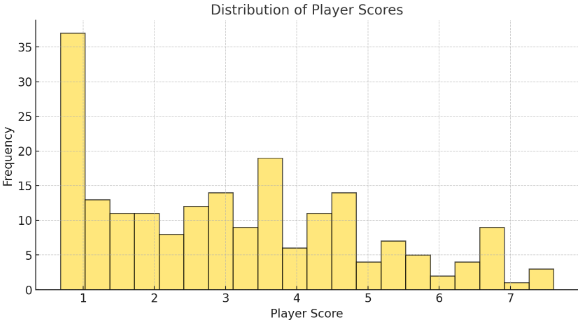
\includegraphics[width=0.45\linewidth]{plot/player_score_distribution.png}
\end{frame}

\begin{frame}{Example: Budget and Forced Assignments}
	\centering
	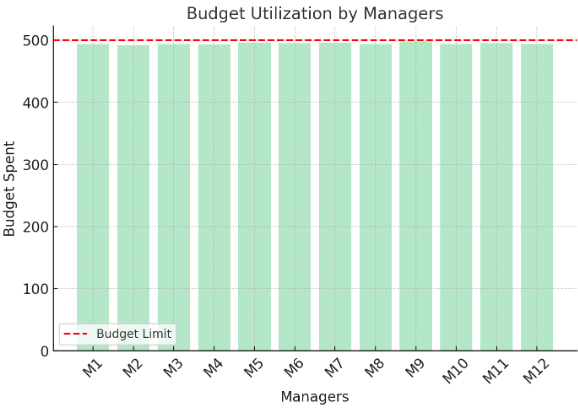
\includegraphics[width=0.45\linewidth]{plot/budget_usage.png}
	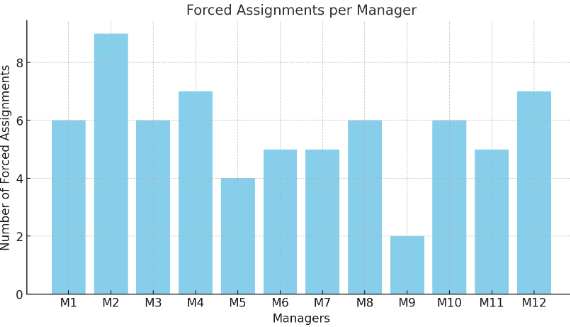
\includegraphics[width=0.45\linewidth]{plot/forced_assignments.png}
\end{frame}

\begin{frame}{Example: Tabular Analyses}
	\scriptsize
	\begin{columns}[T,onlytextwidth]
		\column{0.52\textwidth}

		
		\vspace{0.6em}
		\textbf{Performance by Strategy}

\begin{tabular}{@{}lrrr@{}}
	\toprule
	Str. & Mgr & Avg Score & Avg Forced\\\midrule
	PSO & 4 & 49.9 & 6\\
	\rowcolor{gray!10} DE  & 4 & \textbf{51.8} & 7\\
	ES  & 4 & 44.8 & \textbf{4}\\
	\bottomrule
\end{tabular}

		
		\column{0.48\textwidth}
		\textbf{Manager Recap}
		\begin{tabular}{@{}rrrr@{}}
			\toprule
			Mgr & Forced & Spent & Score\\\midrule
			1 & 6 & 494 & 52.9\\
			2 & 9 & 492 & 51.5\\
			3 & 6 & 494 & 44.5\\
			4 & 7 & 493 & 53.6\\
			5 & 4 & 496 & 49.2\\
			6 & 5 & 495 & 46.0\\
			7 & 5 & 496 & 47.0\\
			8 & 6 & 494 & 55.3\\
			9 & 2 & 498 & 44.2\\
			10& 6 & 494 & 46.6\\
			11& 5 & 495 & 40.0\\
			12& 7 & 494 & 53.2\\
			\bottomrule
		\end{tabular}
		
		\vspace{0.6em}
		\textbf{Player Score Summary}
		\begin{tabular}{@{}lccc@{}}
			\toprule & Best & Worst & Avg\\\midrule
			Score & 12.9 & 0.68 & 2.84\\
			\bottomrule
		\end{tabular}
	\end{columns}
\end{frame}


% ------------------------------------------------------------------ %
\section{Hyper-parameter Tuning}
\begin{frame}{Hyper-parameter Tuning – Design}
	\small
	\begin{columns}[T,onlytextwidth]
		% ---------- LEFT column ------------------------------------------- %
		\column{0.55\textwidth}
		\textbf{Methodology}
		\begin{itemize}
			\item Same 25-player pool, fixed seed, 60 auction turns
			\item Test manager + 1 random rival (guarantees bidding pressure)

		\end{itemize}
		
		\medskip
		\textbf{Cartesian products \(\Rightarrow\) 24 runs}
\begin{itemize}
	\item PSO = 2 inertia weights \(\times\) 2 swarm sizes = \textbf{4} runs
	\item DE = 3 population sizes \(\times\) 2 \(F\) ranges \(\times\) 2 \(CR\) = \textbf{12} runs
	\item ES = 4 \((\mu,\lambda)\) pairs \(\times\) 2 generation counts = \textbf{8} runs
\end{itemize}

	
		% ---------- RIGHT column ------------------------------------------ %
		\column{0.42\textwidth}

\vspace{0.4em}
\textit{Why these ranges?}
\begin{itemize}
	\item Values are the \emph{standard defaults} most cited in the literature  
	(Clerc and Kennedy for PSO, Storn and Price for DE, \(\lambda\!>\!\!\mu\) rule for ES)

	
\end{itemize}
	\end{columns}
\end{frame}

% ------------------------------------------------------------------ %
\begin{frame}{Hyper-parameter Tuning – Results}
	\small
	\begin{columns}[T,onlytextwidth]
		% ---------- LEFT column ------------------------------------------- %
		\column{0.48\textwidth}
\textbf{Best configuration for algorithm}

\centering
\scriptsize
	\begin{center}
	\begin{tabular}{@{}lll@{}}
		\toprule
		\textbf{Alg.} & \textbf{Best h-p} & \textbf{Sum Score} \\
		\midrule
		ES  & $\mu=20,\;\lambda=40,\;ngen=50$          & \textbf{104.7} \\
		DE  & pop$=15,\;F=(0.5,1.0),\;CR=0.7$          & 93.3 \\
		PSO & swarm$=60,\;w=0.9,\;c_{1}=c_{2}=1.49445$ & 92.4 \\
		\bottomrule
	\end{tabular}
\end{center}
		
		\medskip
			\textbf{Parameter grid}

\centering
\scriptsize
\begin{tabular}{@{}l p{6.3cm}@{}}
	\toprule
	PSO &
	$w\in\{0.9,0.5\}$, $c_1=c_2=1.49445$, swarm $\{30,60\}$ \\[2pt]
	DE  &
	pop $\{10,15,20\}$, $F\in\{(0.5,1.0),(0.7,1.2)\}$, $CR\in\{0.7,0.9\}$ \\[2pt]
	ES  &
	$(\mu+\lambda)\in\{(15+30),(15+40),(20+30),(20+40)\}$, $ngen\in\{50,80\}$ \\[2pt]
	\bottomrule
\end{tabular}

		
		% ---------- RIGHT column ------------------------------------------ %
		\column{0.48\textwidth}
		\centering
		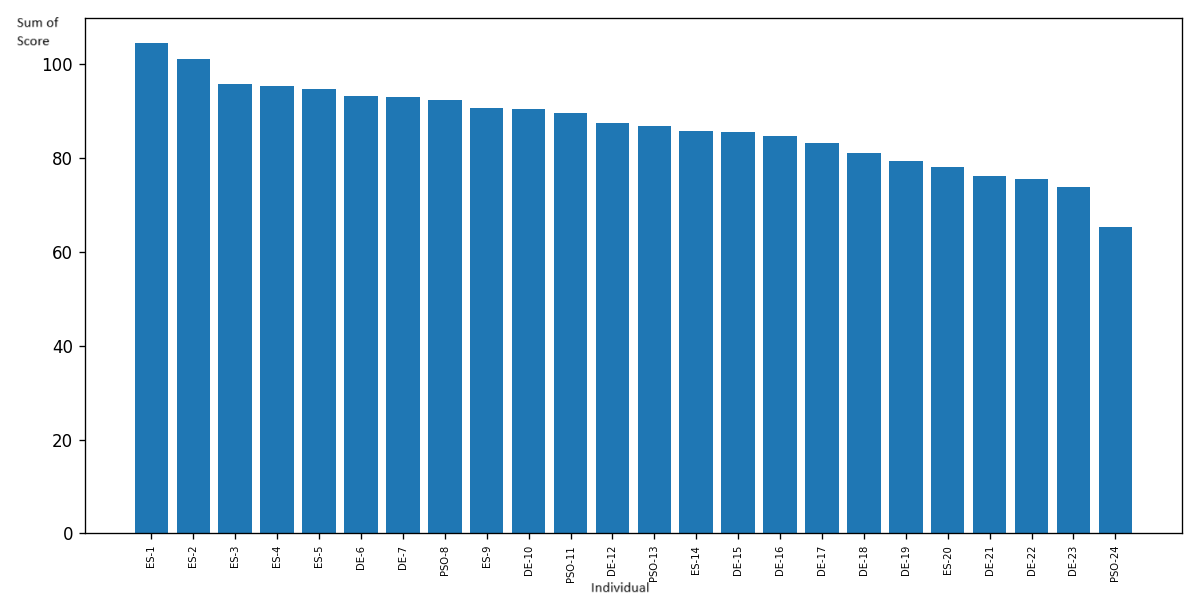
\includegraphics[width=\linewidth]{plot/hyperparam_plot.png}
		\captionof*{figure}{Sum of score for every configuration
			(higher = better).}
	\end{columns}
\end{frame}

\section{Inverse multi–tuning}
\begin{frame}{Inverse multi–tuning/1}
	\small
	\begin{block}{Goal}
     Fit the hyper–parameters
	of \alert{PSO, DE \& ES} so that each auctioned
	roster reproduces a target triple
	$(\text{score},\text{forced picks},\text{leftover})=(100,4,0)$.
	\end{block}
	\medskip
	\[
	\mathcal L(\theta)=|\,\text{score}-100\,|+
	|\,\text{forced}-4\,|+
	|\,\text{leftover}-0\,|
	\qquad\longrightarrow\;\min_{\theta}
	\]
	
	\begin{itemize}
		\item \textbf{Outer optimiser:} 30-particle PSO (40 iterations,
		$\omega\!=\!0.7,\;c_1\!=c_2\!=\!1.5$).
		\item \textbf{Search space:}
		\emph{algo\_id} $\in\{$0:PSO, 1:DE, 2:ES$\}$ + 4 real h-params.
		\item \textbf{Best configuration found:}\\
		DE (pop $=10$, $F\!=[0.7,1.2]$, $CR\!=0.7$)\,$\Rightarrow\,
		\mathcal L_{\min}=0.278$.
	\end{itemize}
	
	%––––––––––––––––––––– LOSS CURVE

\end{frame}

%------------------------------------------------------------
% FRAME 2 – top-5 configurazioni e confronto KPI
%------------------------------------------------------------
\begin{frame}{Inverse multi–tuning/2}
	\small
	\vspace{1ex}
	\centering
	
	%–––––––––––––––– Line chart: loss over iterations
	\textit{Convergence of the inverse tuning process: the total loss $\mathcal{L}$ progressively approaches zero.}
	\medskip
	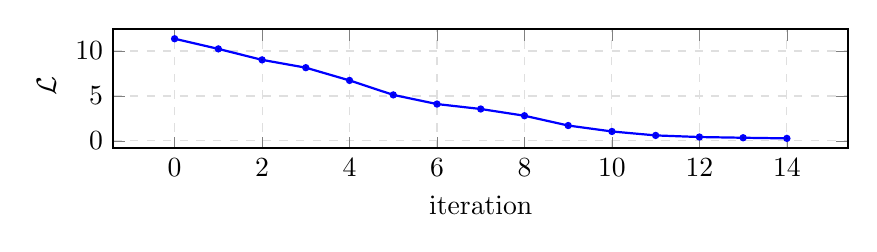
\begin{tikzpicture}
		\begin{axis}[
			height=3.1cm,width=.9\linewidth,
			ylabel={$\,\mathcal L$}, xlabel={iteration},
			ymajorgrids,xmajorgrids,grid style={dashed,gray!25},
			thick,compat=1.18
			]
			\addplot+[mark=*,mark size=.9pt]
			table[x expr=\coordindex, y=loss, row sep=\\]{
				loss\\ 11.37\\ 10.24\\ 9.02\\ 8.15\\ 6.73\\ 5.12\\ 4.10\\
				3.55\\ 2.80\\ 1.71\\ 1.05\\ 0.61\\ 0.43\\ 0.35\\ 0.28\\
			};
		\end{axis}
	\end{tikzpicture}
	
\end{frame}
\begin{frame}{Inverse multi–tuning/3}
	\small
	\vspace{1ex}
	\centering
	
	\begin{columns}[T,onlytextwidth]
		%–––––––––––––––– left: tabella
		\begin{column}{.55\linewidth}
			\textbf{Top-5 trials}\par\medskip
			\footnotesize
			\begin{tabular}{@{}lcccc@{}}
				\toprule
				Alg. & Pop./Swarm / $(\mu,\lambda)$ & $F/(\omega)$ & $CR/c_{1,2}$ & $\mathcal L$\\
				\midrule
				DE  & 10          & 0.7–1.2 & 0.7  & 0.278\\
				ES  & (20,30)     & –       & –    & 1.86\\
				ES  & (20,40)     & –       & –    & 1.98\\
				PSO & 60          & 0.5     & 1.49 & 4.08\\
				DE  & 20          & 0.7–1.2 & 0.7  & 4.20\\
				\bottomrule
			\end{tabular}
			
			\vspace{1ex}
			\textit{Best configurations found during inverse tuning: DE and ES performed best in reproducing the target profile.}
		\end{column}
		
		%–––––––––––––––– right: bar chart
		\begin{column}{.45\linewidth}
			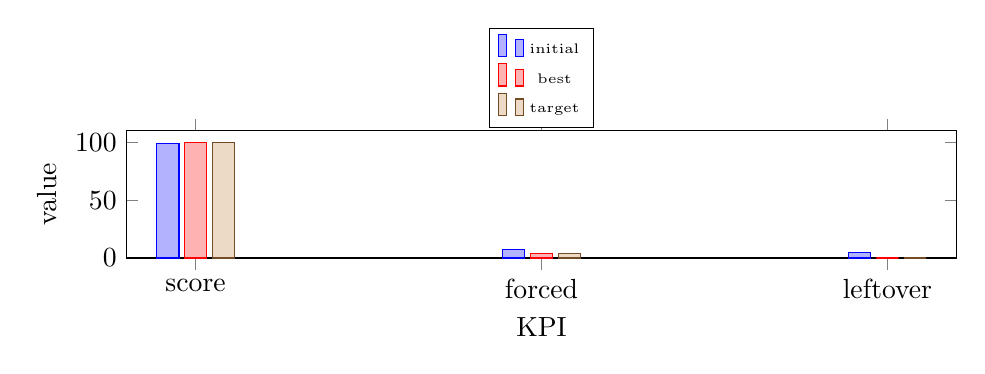
\begin{tikzpicture}
				\begin{axis}[
					ybar, bar width=8pt,
					height=3.2cm,width=\linewidth,
					symbolic x coords={score,forced,leftover},
					ylabel={value}, ymin=0,
					xtick=data, xlabel={KPI},
					legend style={font=\tiny, at={(0.5,1.02)},anchor=south},
					compat=1.18
					]
					\addplot coordinates {(score,99.1) (forced,7) (leftover,5)};
					\addplot coordinates {(score,100.3) (forced,4) (leftover,0)};
					\addplot coordinates {(score,100)   (forced,4) (leftover,0)};
					\legend{initial,best,target}
				\end{axis}
			\end{tikzpicture}
			
			\vspace{1ex}
			\textit{KPI comparison: the best configuration closely matches the target (score 100, 4 forced picks, 0 leftover credits).}
		\end{column}
	\end{columns}
\end{frame}


\end{document}
